\chapter{System Testing}

\section{Introduction}
System testing of software is testing conducted on a complete, integrated system to evaluate the system's compliance with its specified requirements. 
This chapter covers unit and integration testing.
Unit testing can be done by checking each biological property like division, motility and proteolysis.
Integration testing combines all biological properties and checks if it still satisfies the set Mathematical Model.

\section{Unit testing}
In unit testing the smallest testable parts of an application, called units, are individually and independently scrutinized for proper operation. 
Unit test were conducted on units of read configuration, initialization of CA, divide, move, proteolysis, properties of ES and BC, save results and quantify.
Each unit performing its task as expected.

\subsection{Read configuration}
The read configuration module should read values from configuration file, which is being carried out.

\section{Integration testing}
Integration testing is a level of software testing where individual units are combined and tested as a group.

\subsection{Test cases}
Common settings FD Threshold = 0, FD = 1, Doubling Time = 50, Simulation Steps = 1400
\begin{enumerate}
\label{testCases}
 \item Asymmetric Division as $\alpha$ = 0, $\beta$ = 1, $\gamma$ = 100, $\sigma$ = 0, $\mu$ = 0, $\lambda$ = 0. 
 \item Symmetric Division as $\alpha$ = 1, $\beta$ = 1, $\gamma$ = 100, $\sigma$ = 0, $\mu$ = 0, $\lambda$ = 0. 
 \item With Confinement as $\alpha$ 0.5, $\beta$ = 5, $\gamma$ = 200, $\sigma$ = 0.5, $\mu$ = 0, $\lambda$ = 0. 
 \item With Motility as $\alpha$ = 0.5, $\beta$ = 5, $\gamma$ = 200, $\sigma$ = 0.5, $\mu$ = 0.5, $\lambda$ = 0. 
 \item With Proteolysis as $\alpha$ = 0.5, $\beta$ = 5, $\gamma$ = 200, $\sigma$ = 0.5, $\mu$ = 0.5, $\lambda$ = 0.5. 
\end{enumerate}

\subsection{Results and snapshots}
Results obtained for test cases mentioned in ~\ref{testCases}: \\\
  \begin{table}[H]
	\begin{center}
		\begin{tabular}{ |c | c | c | c | c | c | }
			\hline
			\textbf{} & \textbf{Asymmetric}  & \textbf{Symmetric}  & \textbf{Confinement}  & \textbf{Motile}  & \textbf{Proteolysis} \\ \hline
CSC in Zone 1	&	1	&	2179	&	20	&	28	&	1330	\\  \hline
CSC in Zone 2	&	0	&	0	&	0	&	0	&	1054	\\  \hline
CSC in Zone 3	&	0	&	0	&	0	&	0	&	807	\\  \hline
CSC in Zone 4	&	0	&	0	&	0	&	0	&	576	\\  \hline
CSC in Zone 5	&	0	&	0	&	0	&	0	&	448	\\  \hline
TAC in Zone 1	&	0	&	0	&	28	&	175	&	4678	\\  \hline
TAC in Zone 2	&	0	&	0	&	0	&	0	&	5079	\\  \hline
TAC in Zone 3	&	0	&	0	&	0	&	0	&	5112	\\  \hline
TAC in Zone 4	&	0	&	0	&	0	&	0	&	4312	\\  \hline
TAC in Zone 5	&	0	&	0	&	0	&	0	&	2655	\\  \hline
TDC in Zone 1	&	38	&	0	&	20	&	515	&	2087	\\  \hline
TDC in Zone 2	&	0	&	0	&	0	&	1	&	1893	\\  \hline
TDC in Zone 3	&	0	&	0	&	0	&	0	&	2250	\\  \hline
TDC in Zone 4	&	0	&	0	&	0	&	0	&	2276	\\  \hline
TDC in Zone 5	&	0	&	0	&	0	&	0	&	1661	\\  \hline
Total CSC	&	1	&	2179	&	20	&	28	&	4215	\\  \hline
Total TAC	&	0	&	0	&	28	&	175	&	21836	\\  \hline
Total TDC	&	38	&	0	&	20	&	516	&	10167	\\  \hline
Total Cells	&	39	&	2179	&	68	&	719	&	36218	\\  \hline
CSC Percentage	&	0.0256	&	1	&	0.2941	&	0.0389	&	0.1163	\\  \hline
ES in Zone 1	&	0	&	0	&	4065	&	4126	&	0	\\  \hline
ES in Zone 2	&	0	&	0	&	3982	&	3997	&	0	\\  \hline
ES in Zone 3	&	0	&	0	&	4168	&	4204	&	0	\\  \hline
ES in Zone 4	&	0	&	0	&	4074	&	3976	&	186.349	\\  \hline
ES in Zone 5	&	0	&	0	&	3826	&	3759	&	1138.28	\\  \hline
Total ES	&	0	&	0	&	20115	&	20062	&	1324.629	\\  \hline
		\end{tabular}
		\caption{Quantification of test cases}
		\label{Tbl_quantification_of_test_cases}
	\end{center}
\end{table} 

  
\subsection{Asymmetric division}
Only asymmetric division should result in only one CSC, rest of BC will be TAC or TDC, 
which is verified in (Table \ref{Tbl_quantification_of_test_cases} Asymmetric) and (Figure \ref{TestCaseResults} A).

\subsection{Symmetric division}
Only symmetric division should result in all BC being CSC, 
which is verified in (Table \ref{Tbl_quantification_of_test_cases} Symmetric) and (Figure \ref{TestCaseResults} B).
  
\subsection{With confinement}
\label{withConfinementTestCase}
With ECM confinement should result in less proliferation, number of BC and zones proliferated to is lesser than with motility case (~\ref{withMotilityTestCase}), 
which is verified in (Table \ref{Tbl_quantification_of_test_cases} Confinement) and (Figure \ref{TestCaseResults} C). 
No change in ES, and around 20000 number of ES as $\sigma$\ =\ 0.50 

\subsection{With motility}  
\label{withMotilityTestCase}
BC with motility but without proteolysis propensity, 
but BCs will have higher proliferation so BCs found in outer zones also as compared to with confinment case (~\ref{withConfinementTestCase}), 
which is verified in (Table \ref{Tbl_quantification_of_test_cases} Motility) and (Figure \ref{TestCaseResults} D).
No change in ES, and around 20000 number of ES as $\sigma$\ =\ 0.50
  
\subsection{With proteolysis}  
\label{withProteolysisTestCase}
There should be change in ES count as BC now have ECM proteolysis capabilities as 
compared to confinement(~\ref{withConfinementTestCase}) and motility case(~\ref{withMotilityTestCase}) where ES count does not change, 
This is verified in (Table \ref{Tbl_quantification_of_test_cases} Proteolysis) and (Figure \ref{TestCaseResults} E).

\begin{figure}[H]
	  \centering
	  \fbox{ 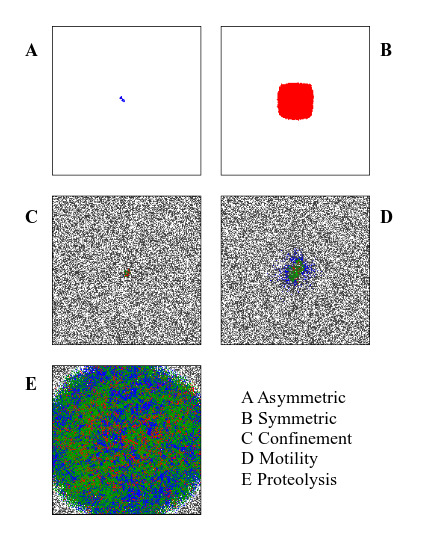
\includegraphics[scale=0.50]{images/TestCaseResults.png} }
	  \caption{Test case results}
	  \label{TestCaseResults}
  \end{figure}

\section{Conclusion}  
Unit test cases covered testing of basic biological properties and integration testing of collection of the basic biological properties as one system.
Test cases are matching expected results of biological settings of intrinsic parameters, with confinement, with motility and with proteolysis.

